\documentclass{../../templates/amendment}
\usepackage{blindtext}
\usepackage[ngerman]{babel}
\usepackage{graphicx}
\usepackage{subcaption}
\usepackage[skip=2pt,font=small]{caption}

% \usepackage{showframe}
\occasion[Berzirksvertretung]{Bezirksvertretung Innenstadt-West}
\date{29. Dezember 2024}
\setcounter{nthantrag}{1}
\begin{document}

\begin{boxed}{Sportanlage Am Tremonipark / Haldenstr.}{Jan Lucas Brause, Maximilian Sackel}
    Die neue Calisthenicsanlage im Tremoniapark bildet in Kombination mit dem Basket- und Fußballplatz einen Treffpunkt für alle Generationen und einen Querschnitt der Bevölkerung.
    Neben spielenden Kindern auf dem Boltzplatz und Jugendlichen auf dem Basketballplatz finden sich dort genauso Erwachsene, die ihre Zeit am Calisthenics Park zum Trainieren nutzen.
    Ebenso wird die Sportanlage von vielen Studierenden und jungen Berufstätigen als unverbindliche und kostenlose Trainingsmöglichkeit äußerst gut angenommen.
    Zudem haben sich in Dortmund bereits Sportvereine mit Calisthenics als Schwerpunkt gebildet, welche auch diese Sportanlage für ihren Trainingsmittelpunkt nutzen und somit das angeleitete Sportangebot und die sozialen Strukturen in Dortmund stärken.

    Die Nutzung der Sportanlagen ist jedoch deutlich auf die Sommermonate limitiert, da bei frühem Einbruch der Dunkelheit in den Wintermonaten sowohl der Bolzplatz, der Basketballplatz und die Trainingsanlage nicht beleuchtet werden.
    Einfache Dinge, wie beispielsweise nicht einsehbarer Kot auf Wegen können bereits die Nutzung beeinträchtigen.
    Hinzu kommen schwerwiegende Vorfälle mit Schreckschusswaffen, Drogendelikten oder aggressiven und gereizten Obdachlosen.
    Generell sind die Sportplätze schwer einsehbar und beschriebene Personen nutzen regelmäßig anliegende Gebüsche und das Unterholz und tauchen aus Sicht der Sport- und Trainingsanlagen aus dem Nichts auf.
    Auch Vandalismus und Graffitis an den teuren Sportgeräten und Sportplätzen wird durch eine Beleuchtung vorgebeugt.

    Eine Beleuchtung bspw. mit Zeitschaltuhr verlängert die Nutzungsdauer und sorgt durch die Anwesenheit von Trainierenden und Sportlern dafür, dass die Fläche unattraktiver für benannte dubiose Tätigkeiten wird.
    Des Weiteren wird durch eine Beleuchtung in den Abendstunden ein ausgeweitetes Sportangebot für zeitlich und finanziell eingeschränkte Bürger geschaffen.

    Eine Lichtverschmutzung besteht nicht, da es sich um urbanes Gebiet handelt und einige Hundehalter ihre Tiere ohne Leine laufen lassen.
    Aufgrund der Entfernung zu Wohnhäusern ist eine Störung der Anwohner durch die Beleuchtung ausgeschlossen.
    Bei einer ähnlichen Spiel- und Sportanlage an der Düsterstraße in Dortmund Körne wurde bereits eine Beleuchtung ohne das Verlegen von Stromleitungen im Erdreich mittels einer integrierten Solareinheit realisiert.

    Zudem möge die Bezirksvertretung beschließen im Sinne der beschlossenen Richtlinie (EU) 2020/2184 des Europäischen Parlaments und des Rates vom 16. Dezember 2020 über die Qualität von Wasser für den menschlichen Gebrauch (ABl. L 435 vom 23.12.2020, S. 1) zur Bereitstellung von kostenlosem Trinkwasser im öffentlichen Raum einen Trinkwasserbrunnen in direkter Nähe zu den Sportgeräten aufzustellen.
    Der Gesetzentwurf setzt die Regelung nach Artikel 16 Absatz 2 Satz 1 der Richtlinie um, wonach die Mitgliedstaaten sicherstellen, dass Leitungswasser zur Nutzung als Trinkwasser an öffentlichen Orten durch Innen- und Außenanlagen bereitgestellt wird, soweit dies technisch durchführbar und unter Berücksichtigung des Bedarfs und der örtlichen Gegebenheiten, wie Klima und Geografie, verhältnismäßig ist (Paragraf 50 Absatz 1 Satz 2 WHG neu).

    Im Anhang sind Abbildungen für eine bessere Einsicht der Sachlage angefügt.
    Einen Ortstermin zu einer Machbarkeitsstudie, sowie die Bündelung weiterer möglicher Verbesserung und Sanierungsvorschläge, halten wir für sinnvoll.

    Über eine Bearbeitung und positive Rückmeldung würden wir uns sehr freuen.
    Selbstverständlich stehen wir gerne für Rückfragen und zur Terminvereinbarung zur Verfügung.

    \begin{figure}[htpb]
        \centering
        \begin{subfigure}[]{0.49\textwidth}
            \begin{center}
                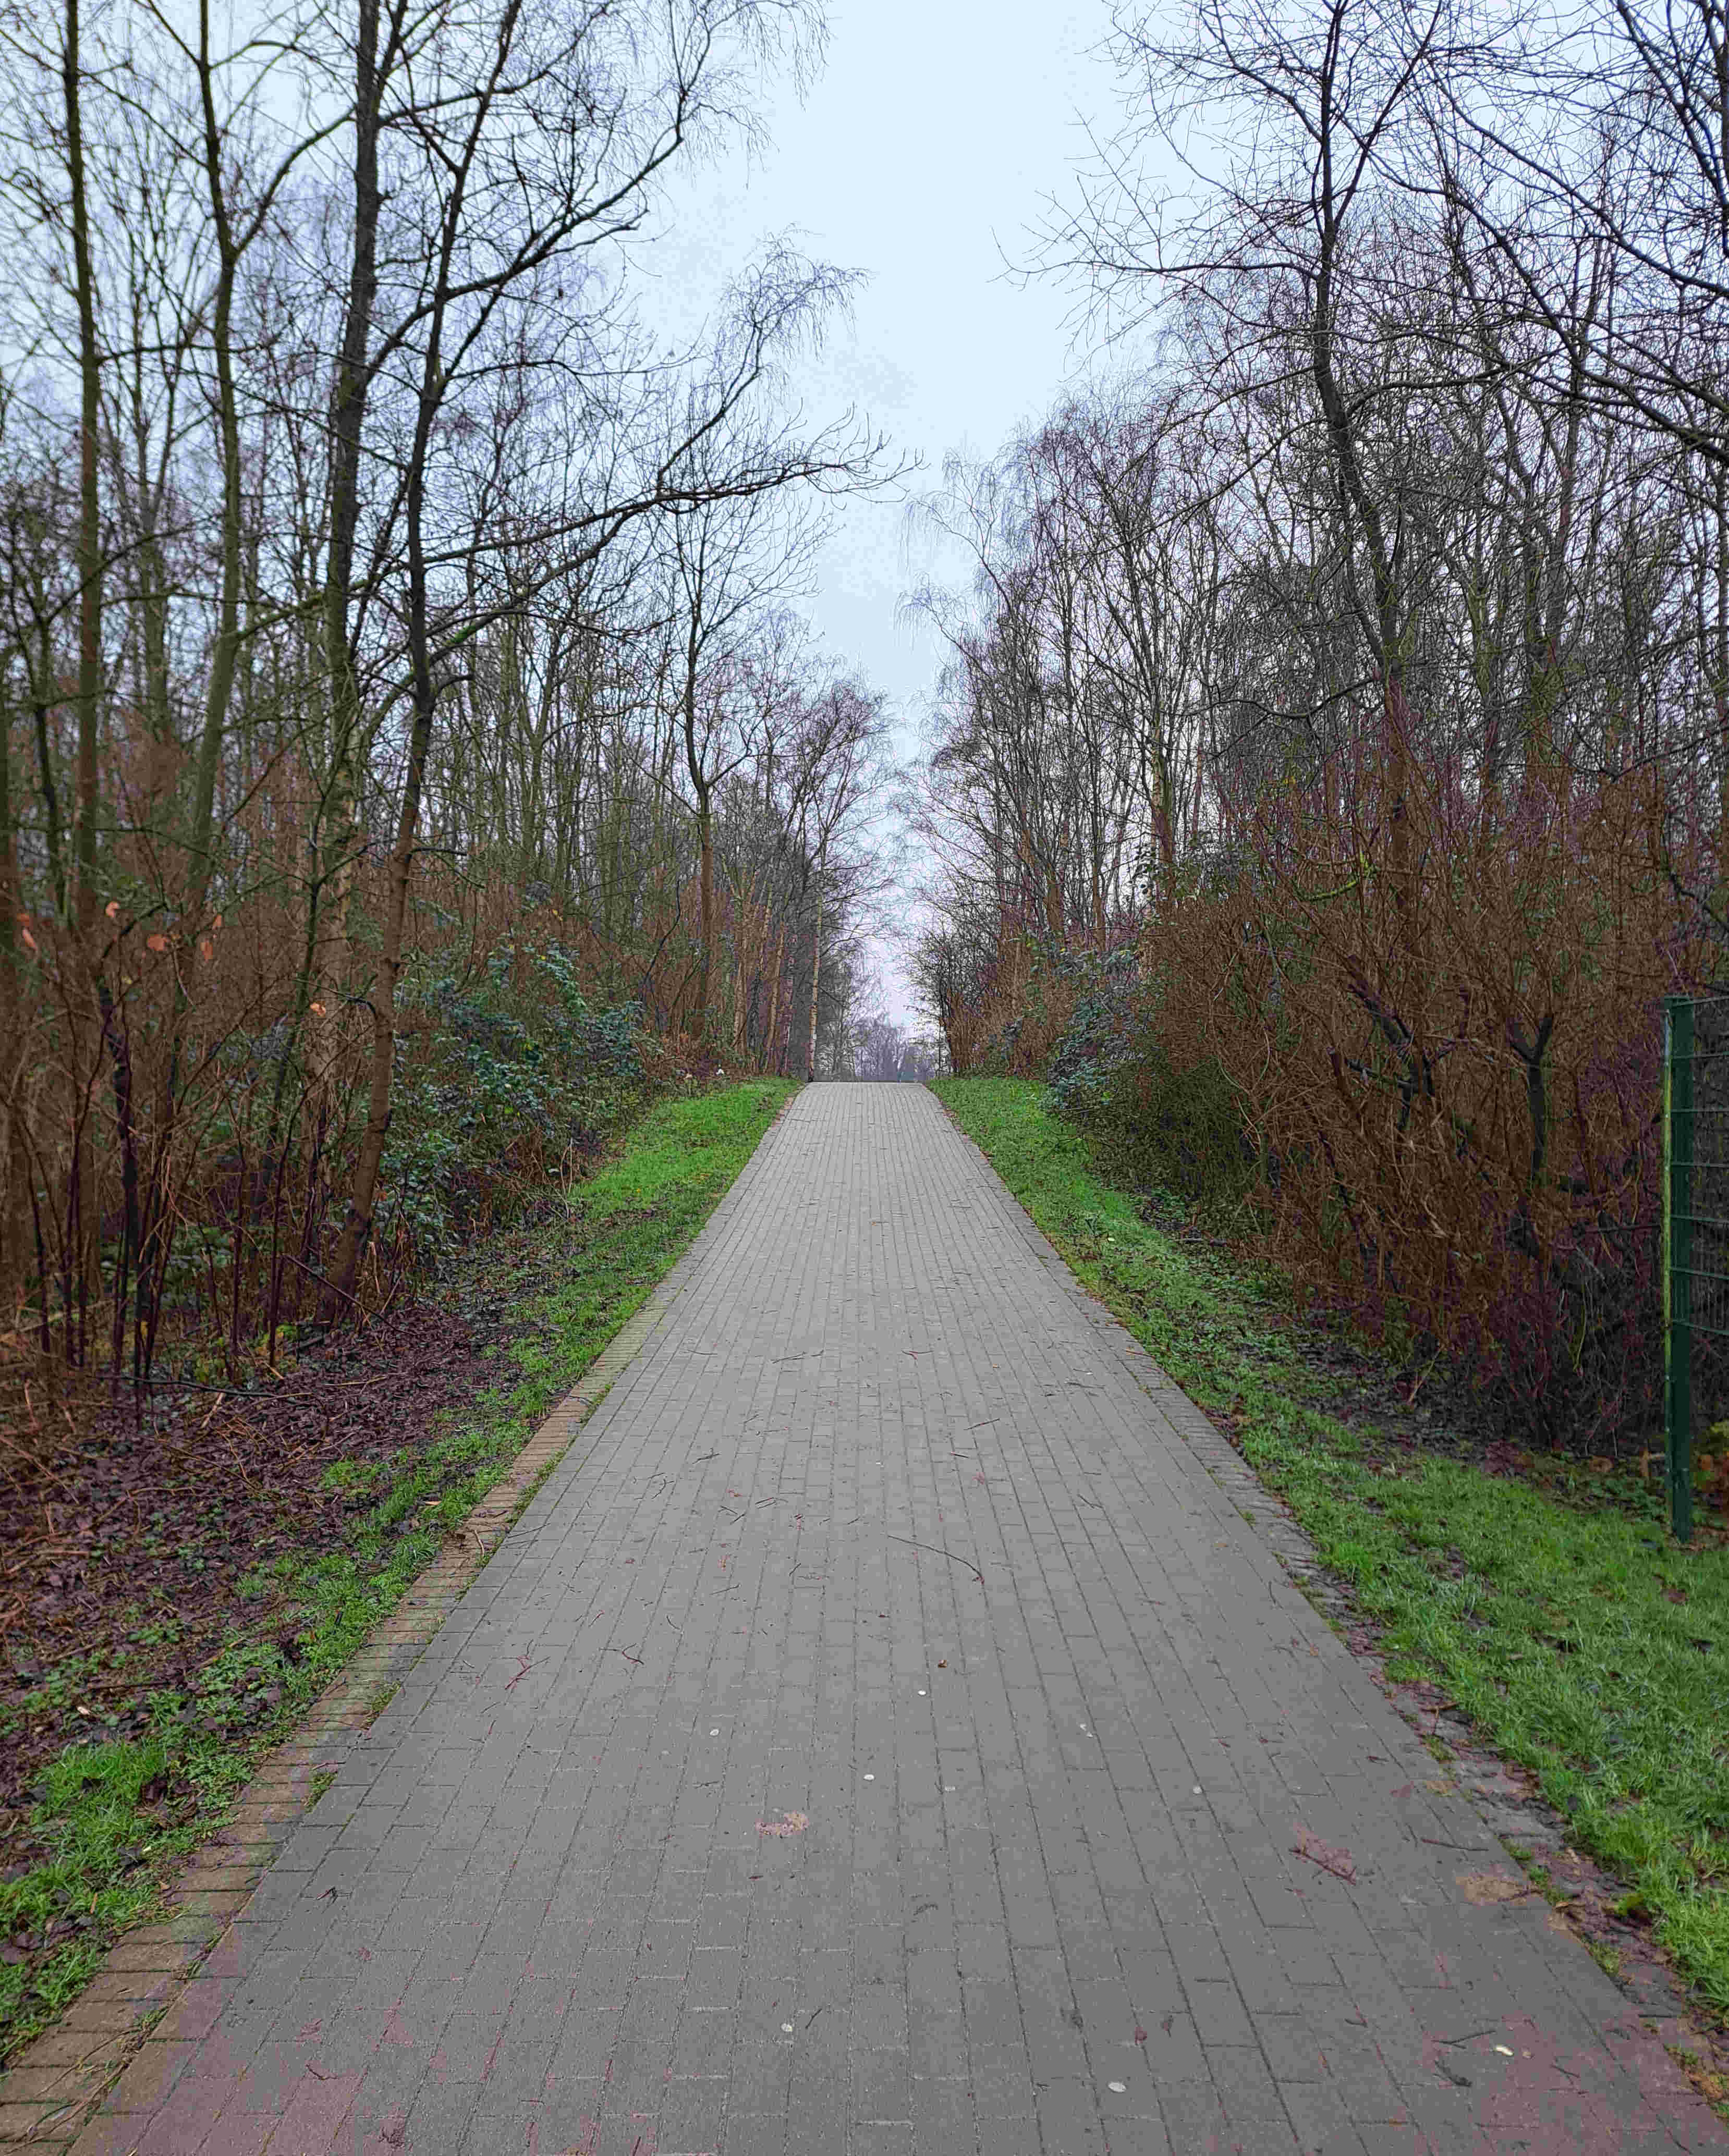
\includegraphics[width=\linewidth]{pictures/photo1.jpg}
                \caption{Calisthenics-Anlage}%
            \end{center}
        \end{subfigure}
        \begin{subfigure}[]{0.49\textwidth}
            \begin{center}
                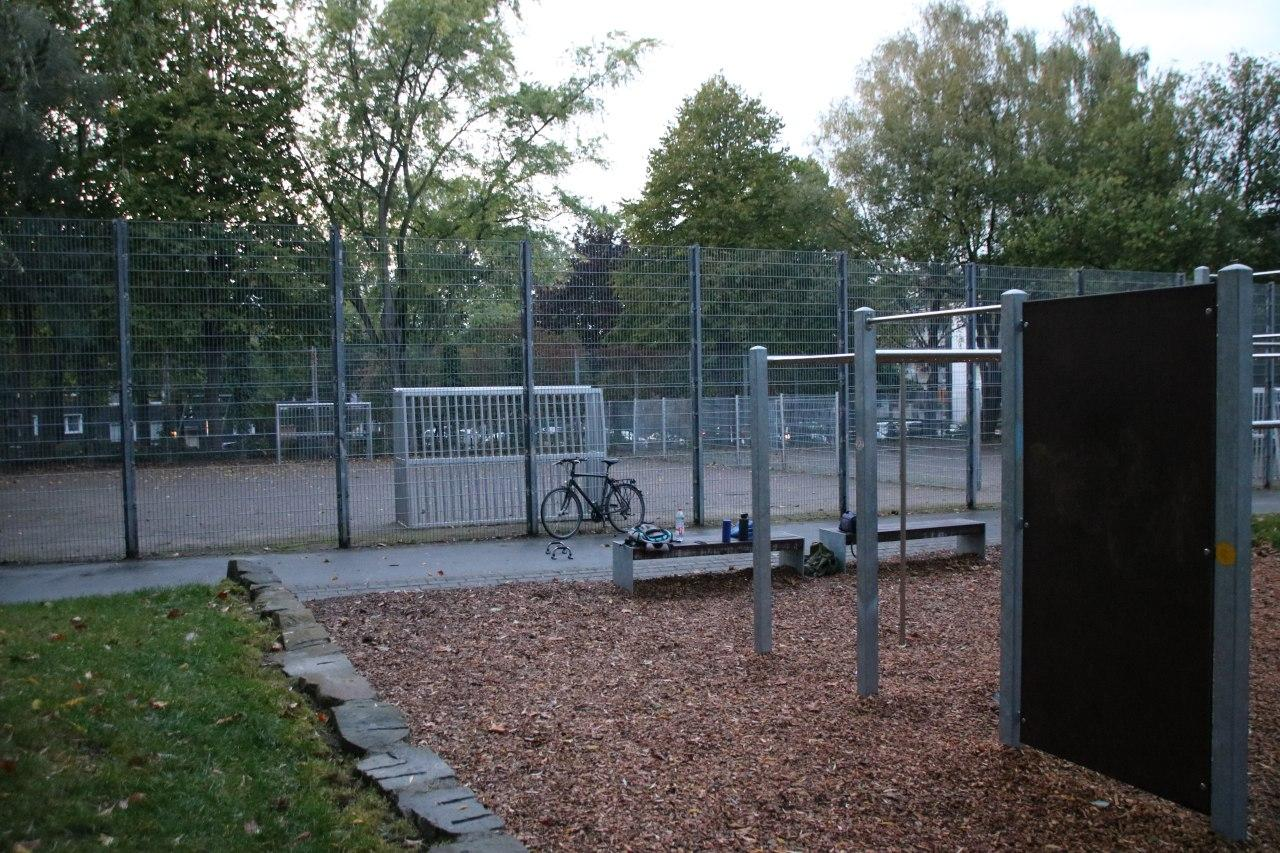
\includegraphics[width=\linewidth]{pictures/photo3.jpg}
                \caption{Angrenzender Boltzplatz}%
            \end{center}
        \end{subfigure}
        \caption{Verbesserungsbedürftige Ausleuchtungssituation begrenzt die
            Nutzungsdauer in den Wintermonaten und schafft durch schlechte Einsicht
        einen Angstraum.}
    \end{figure}

    \begin{figure}[htpb]
        \centering
        \begin{subfigure}[]{0.49\textwidth}
            \begin{center}
                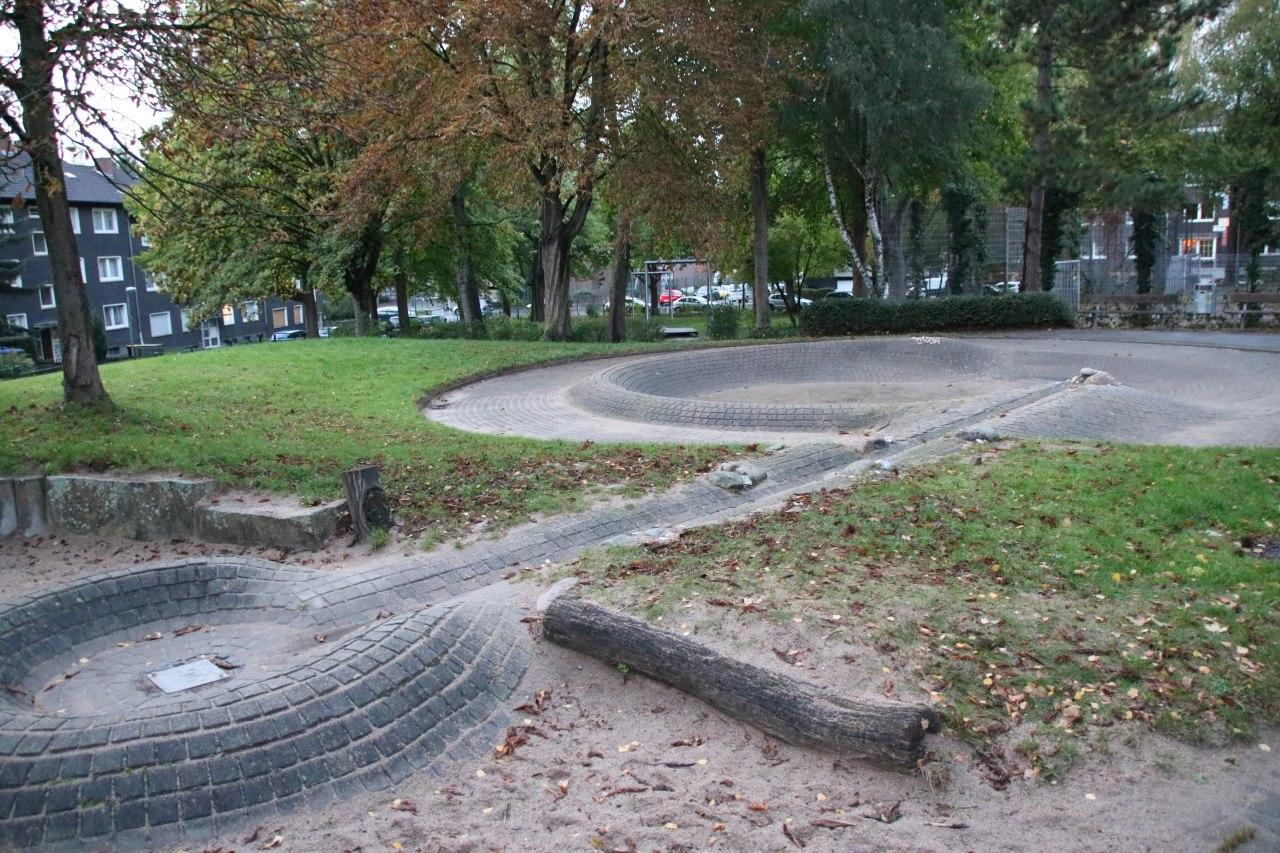
\includegraphics[width=\linewidth]{pictures/photo2.jpg}
                \caption{Wasserspielplatz}%
            \end{center}
        \end{subfigure}
        \begin{subfigure}[]{0.49\textwidth}
            \begin{center}
                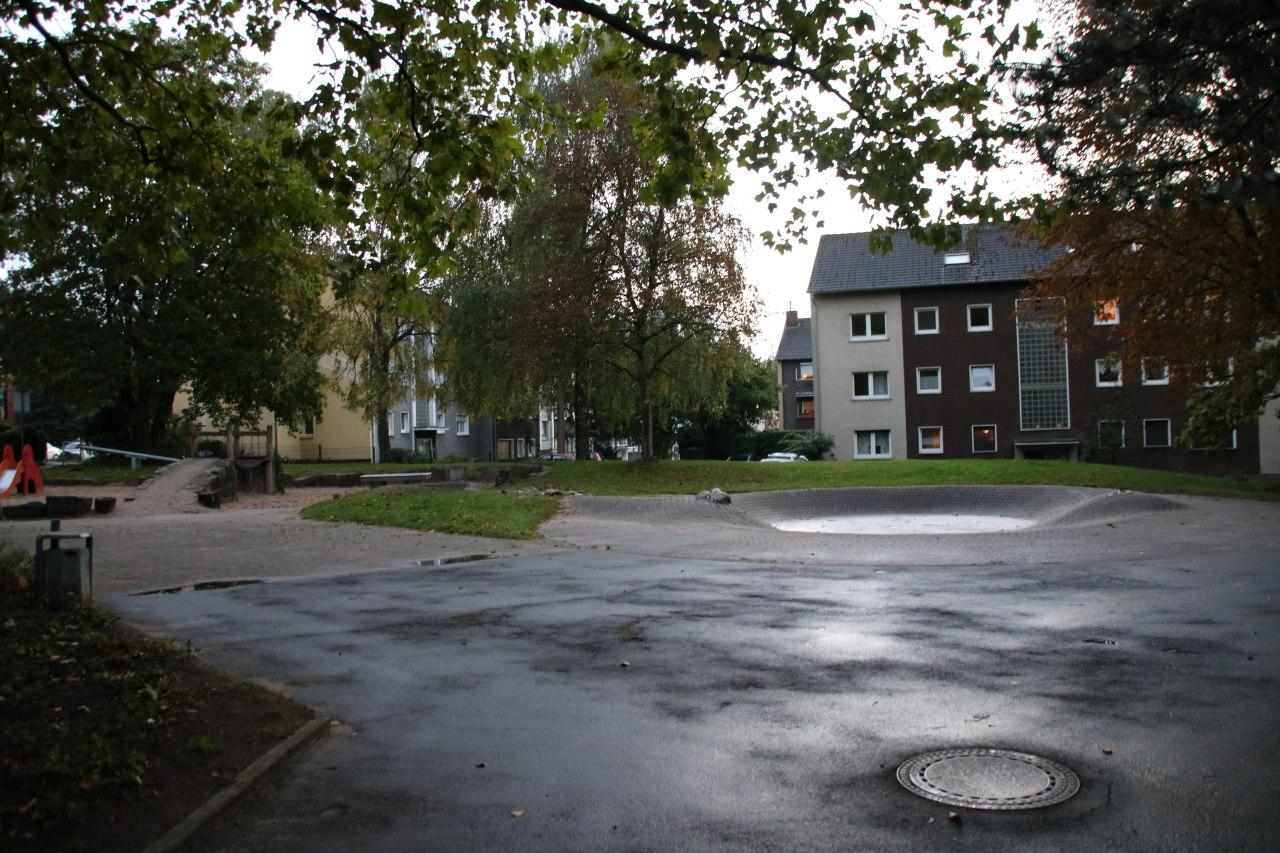
\includegraphics[width=\linewidth]{pictures/photo4.jpg}
                \caption{ungenutzte Fläche}%
            \end{center}
        \end{subfigure}
        \caption{Erweiterung des bestehenden Wasserspielplatzes durch einen
            Brunnen, würde die Trinkwasserversorgung für spielende Kinder, Eltern
        sowie Trainierende sicherstellen.}
    \end{figure}
\end{boxed}

\end{document}
